\documentclass[a4paper]{article}

\usepackage[utf8]{inputenc}
\PassOptionsToPackage{hyphens}{url} % zodat url's ook afgekapt worden
\usepackage{hyperref}
\usepackage[dutch]{babel}
\usepackage{graphicx}
\graphicspath{{img/}}
\usepackage{algorithm}
\usepackage{algorithmic}
\usepackage[toc,page]{appendix}
\usepackage{mathtools}
\usepackage{tikz}
\usepackage{tocbibind}
\usepackage{float}
\usepackage{framed}
\usepackage{parskip}
\usepackage{listings}
\usepackage{color}
\usepackage{pdfpages}
\usepackage{pdflscape}
\usepackage{todonotes}
\usepackage{tabularx}
\usepackage{usecases}

\begin{document}
%%%%%%%%%%%%%%%%%%%%%%%%%%%%%%%%%%%%%%%%%
% University Assignment Title Page 
% LaTeX Template
% Version 1.0 (27/12/12)
%
% This template has been downloaded from:
% http://www.LaTeXTemplates.com
%
% Original author:
% WikiBooks (http://en.wikibooks.org/wiki/LaTeX/Title_Creation)
%
% License:
% CC BY-NC-SA 3.0 (http://creativecommons.org/licenses/by-nc-sa/3.0/)
% 
% Instructions for using this template:
% This title page is capable of being compiled as is. This is not useful for 
% including it in another document. To do this, you have two options: 
%
% 1) Copy/paste everything between \begin{document} and \end{document} 
% starting at \begin{titlepage} and paste this into another LaTeX file where you 
% want your title page.
% OR
% 2) Remove everything outside the \begin{titlepage} and \end{titlepage} and 
% move this file to the same directory as the LaTeX file you wish to add it to. 
% Then add \input{./title_page_1.tex} to your LaTeX file where you want your
% title page.
%
%%%%%%%%%%%%%%%%%%%%%%%%%%%%%%%%%%%%%%%%%

%----------------------------------------------------------------------------------------
%	PACKAGES AND OTHER DOCUMENT CONFIGURATIONS
%----------------------------------------------------------------------------------------
\begin{titlepage}
\pagestyle{empty}
\newcommand{\HRule}{\rule{\linewidth}{0.5mm}} % Defines a new command for the horizontal lines, change thickness here

\center % Center everything on the page
 
%----------------------------------------------------------------------------------------
%	HEADING SECTIONS
%----------------------------------------------------------------------------------------

\textsc{\LARGE Universiteit Hasselt}\\[1.5cm] % Name of your university/college
\textsc{\Large Software Engineering}\\[0.5cm] % Major heading such as course name
\textsc{\large Requirements analyse }\\[0.5cm] % Minor heading such as course title
% \textsc{\LARGE Modulo}\\[0.5cm] % Minor heading such as course title

%----------------------------------------------------------------------------------------
%	TITLE SECTION
%----------------------------------------------------------------------------------------

\HRule \\[0.4cm]
%{ \huge \bfseries Managementsysteem \\ Deeltijds Onderwijs }\\[0.2cm] % Title of your document
{ \huge \bfseries Modulo \\ \vspace{-0.4em} ----- \vspace{-0.4em}\\ Managementsysteem \\ Deeltijds Onderwijs }\\[0.2cm] % Title of your document
\HRule \\[1.5cm]
 
%----------------------------------------------------------------------------------------
%	AUTHOR SECTION
%----------------------------------------------------------------------------------------

\begin{minipage}{0.4\textwidth}
\begin{flushleft} \large
\emph{Auteurs:}\\
Vincent \textsc{Drozdzyniak} % Your name
Hendrik \textsc{Lievens} \\ 
Martijn \textsc{Maes} \\
Reinaert \textsc{Van de Cruys} \\
Michiel \textsc{Vanmunster} \\
Jens \textsc{Vannitsen}
\end{flushleft}
\end{minipage}
~
\begin{minipage}{0.4\textwidth}
\begin{flushright} \large
% \emph{Promotor:} \\
% Prof. dr. Frank \textsc{Neven}\\ % Supervisor's Name
% \vspace{4mm}
\emph{Begeleider:} \\
Robin \textsc{Marx}
\end{flushright}
\end{minipage}\\[2.5cm]

% If you don't want a supervisor, uncomment the two lines below and remove the section above
%\Large \emph{Author:}\\
%John \textsc{Smith}\\[3cm] % Your name


%----------------------------------------------------------------------------------------
%	DATE SECTION
%----------------------------------------------------------------------------------------

{\large 17 maart 2016}\\[2cm] % Date, change the \today to a set date if you want to be precise

%----------------------------------------------------------------------------------------
%	LOGO SECTION
%----------------------------------------------------------------------------------------


\includegraphics[width=0.4\textwidth]{UH_logo}\\[2cm] % Include a department/university logo - this will require the graphicx package
 
%----------------------------------------------------------------------------------------

\vfill % Fill the rest of the page with whitespace

\end{titlepage}

\tableofcontents
\newpage

\section{Preface}
Dit document is bedoeld voor het personeel van het Technisch Instituut Heilig Hart te Hasselt \cite{TIHH} zijnde de opdrachtgevers, het onderwijsteam en het ontwikkelingsteam van Modulo. In dit document worden alle vereisten van het softwarepakket geanalyseerd.

\section{Inleiding}
Modulo is een Managementsysteem voor het Deeltijds Onderwijs (MDO) dat gebruikt kan worden in alle onderwijsinstellingen waar het Deeltijds Beroepssecundair Onderwijs (DBSO) \cite{DBSO} als onderwijsvorm wordt gehanteerd. Dit omvat alle Centra voor Deeltijds Onderwijs (CDO) \cite{CDO} alsook het Syntra-netwerk \cite{Syntra}. Met de invoering van het duaal leren \cite{Duaal_leren} zal Modulo ook in alle technische en beroepsrichtingen gebruikt kunnen worden.

Modulo kan informatie over leerlingen en personeel bijhouden en de klassen en graden van een school beheren. De belangrijkste component van het softwarepakket is het puntensysteem, waarmee leerkrachten de voortgang van leerlingen kunnen bijhouden. Dit systeem laat ook toe om automatisch overzichtelijke rapporten te genereren.

Het softwarepakket omvat ook een digitale agenda, een geïntegreerd berichten- en meldingensysteem, een online bestandsysteem en een uploadzone voor taken. Er worden verschillende types van gebruikers ondersteund, namelijk beheerder, leerkracht, leerling en ouder. De focus van het softwarepakket ligt op gebruiksvriendelijkheid, in het bijzonder overzichtelijkheid.

In sectie \ref{sec:user_req} worden alle vereisten van het softwarepakket tegenover de gebruiker besproken. Er wordt een uitgebreide lijst van vereiste functionaliteiten gegeven, alsook een analyse van het gebruik, de mogelijkheden voor ondersteuning en de juridische aspecten van het softwarepakket. Sectie \ref{sec:systeemarchitectuur} vormt een uiteenzetting van de implementatie en de gekozen technologieën om het softwarepakket te implementeren en in sectie \ref{sec:use_cases} wordt dieper ingegaan op de concrete stappen die verschillende types gebruikers moeten nemen om bepaalde acties uit te voeren. In de appendices tenslotte kunnen mockups gevonden worden van de web- en de mobiele applicatie.

\section{Woordenlijst} % voor de klant
\def\arraystretch{1.8}
\begin{tabularx}{\textwidth}{l | X}
    Term & Definitie \\
    \hline \hline
    MDO &`Managementsysteem voor het Deeltijds Onderwijs' is het antwoord op de vraag ``Wat is Modulo?''. Het is een softwarepakket voor het beheren van de persooneels- en leerlingengegevens binnen het DBSO. \\
    \hline
    DBSO & `Deeltijds Beroepssecundair Onderwijs', of kortweg `deeltijds onderwijs', is een onderwijsvorm waarin leerlingen leren op school combineren met leren op werkplekken. Een lesweek bestaat uit 8 uur BGV en 7 uur PAV, de rest van de tijd brengen de leerlingen door op de werkvloer. \cite{DBSO} \\
    \hline
    CDO & `Centrum voor Deeltijds Onderwijs' is een school die DBSO als onderwijsvorm hanteert. De opdrachtgever voor Modulo, het Technisch Instituut Heilig Hart te Hasselt \cite{TIHH}, is hier een voorbeeld van. \cite{CDO} \\
    \hline
    BGV & `Beroepsgerichte Vorming' is het vak binnen het DBSO dat alle beroepsspecifieke competenties voor een opleiding omvat en zo de leerlingen alle kennis en vaardigheden bijbrengt die ze op de werkvloer nodig hebben. \\
    \hline
    PAV & `Project Algemene Vorming' of `Project Algemene Vakken' is het vak binnen het DBSO dat in alle doelstellingen van de 2de en 3de graad omvat, zodat de leerlingen hun diploma secundair onderwijs kunnen behalen. \\
    \hline
    Competentie & Het certificaat dat door middel van BGV verkregen kan worden, bestaat uit een verzameling deelcertificaten. Ieder deelcertificaat bestaat uit een lijst van competenties, vastgelegd door de Vlaamse overheid, die de leerlingen allemaal moeten halen om het deelcertificaat te verkrijgen. Een deelcertificaat kan op andere deelcertificaten voortbouwen, die dan ook in volgorde behaald moeten worden. \cite{Competenties} \\
    \hline
    Doelstelling & Een doelstelling is een module binnen PAV die bepaald wordt door de eindtermen voor het secundair onderwijs van de Vlaamse overheid. leerlingen moeten alle doelstellingen halen alvorens ze het diploma secundair onderwijs kunnen ontvangen. Een doelstelling kan bestaan uit andere doelstellingen, die dan opnieuw allemaal behaald moeten worden. \cite{Doelstellingen} \\
\end{tabularx}

\section{User requirements}  \label{sec:user_req}% voor de klant

\subsection{Functionele requirements}
\begin{enumerate}
% algemeen
\item Het systeem moet toelaten om gebruikers toe te voegen en te verwijderen.
\item Het systeem moet toelaten om aan een gebruiker een rol (leerkracht, leerling, beheerder, ouder) toe te kennen.
\item Het systeem moet toelaten om in te stellen of een leerling al dan niet actief is.
\item Het systeem moet toelaten om de persoonlijke informatie van een leerling aan te passen.
\item Het systeem moet toelaten om leerlingen in te kunnen schrijven.
\item Het systeem moet toelaten om inschrijvingsgeralteerde informatie van een leerling aan te passen.
\item Het systeem moet toelaten om informatie over de leerkrachten te bewerken.
\item Het systeem moet toelaten om informatie van een beheerder te wijzigen.
\item Het systeem moet toelaten om graden toe te voegen, te verwijderen en te bewerken.
\item Het systeem moet toelaten om opleidingen toe te voegen, te verwijderen en te bewerken.
\item Het systeem moet toelaten om subklassen aan een klas/richting toe te voegen, te verwijderen en te bewerken.  % klas voor in de voormiddag, klas voor in de namiddag
\item Het systeem moet toelaten om leerlingen aan een subklas toe te voegen en te verwijderen.
% PAV
\item Het systeem moet toelaten om, in het algemeen, PAV-competenties toe te voegen, te verwijderen en te bewerken.
\item Het systeem moet toelaten om projecten/vakthema's aan een klas toe te kennen. Deze worden opgebouwd uit doelstellingen.
\item Het systeem moet toelaten om taken toe te voegen aan vakthema's.
% BGV
\item Het systeem moet toelaten om BGV-certificaten toe te voegen, te verwijderen en te bewerken.
\item Het systeem moet toelaten om deelcertificaten aan een BGV-certificaat toe te voegen, te verwijderen en te bewerken.
% algemeen (scores)
\item Het systeem moet toelaten om een score (A,I,V) toe te kennen aan een competentie binnen een vakthema, voor een leerling.  % PAV
\item Het systeem moet toelaten om een score (A,I,V) toe te kennen aan een competentie binnen een deelcertificaat, voor een leerling.  % BGV
\item Het systeem moet automatisch het behalen van een competentie blokkeren, indien deze reeds drie maal verworven (score V) werd.  % 3x verwerven == behaald
\item Het systeem moet het verloop van het jaar kunnen weergeven (De score toekenning van een doelstelling in een periode)
\item Het systeem moet toelaten om een beschrijving te geven bij het verwerven van een competentie.
\item Het systeem moet toelaten om een ingevuld rapport te genereren, voor een leerling.
\item Het systeem moet toelaten om de houdingen/attitudes van de leerlingen in te vullen.
% algemeen
\item Het systeem moet toelaten om informatie over de school aan te passen.
\item Het systeem moet toelaten om werkgevers waar de school mee samenwerkt toe te voegen en te verwijderen, en hun informatie aan te passen.
\item Het systeem moet toelaten om een werkgever (waar de school mee samenwerkt) aan een leerling toe te wijzen.
\item Het systeem moet toelaten om een contract te genereren voor de samenwerking tussen leerling en werkgever.
\item Het systeem mag toelaten om berichten te versturen naar anderen.  
\item Het systeem mag toelaten om bestanden te uploaden. 
\item Het systeem moet een agenda voorzien.
\item Het systeem moet bijhouden hoe vaak en wanneer ouders aanmelden.
\end{enumerate}

\subsection{Usability}
De gebruikersinterface is een uitgesproken belangrijk onderdeel van Modulo. Omdat het om een managementsysteem gaat, staat of valt de bruikbaarheid van het softwarepakket met diens overzichtelijkheid. Voor zowel de leerling als de leerkracht en de beheerder zijn duidelijkheid en een vlotte werking essentieel. Ook consistentie is van belang, in het bijzonder omdat het softwarepakket op meerdere platformen beschikbaar is.

\subsection{Reliability}
Zowel de webapplicatie als de mobiele applicatie zijn slechts interfaces naar de back-end. Bijgevolg is uptime van de back-end server essentieel voor de reliability van het softwarepakket. Om die reden zal hosting van deze server uitbesteed worden aan een gespecialiseerd bedrijf met een hoge uptime garantie, dat deze taak vermoedelijk goedkoper en betrouwbaarder zal uitvoeren dan het ontwikkelingsteam zelf.

\subsection{Performance}
Op het vlak van performantie zijn er geen specifieke vereisten, enkel dat op alle acties een snelle ($<$ 2 sec.) respons volgt. Op die manier komt de gebruiksvriendelijkheid nooit onder de snelheid van de software te lijden. De database moet wel snel genoeg zijn om ook bij grote scholen, bestaande uit duizenden leerlingen, vlot te blijven werken. Hiervoor kan er nood zijn aan snelle hardware en enkele gerichte optimalisaties.

\subsection{Supportability}
Het softwarepakket moet makkelijk uitbreidbaar en eenvoudig te onderhouden zijn. In het geval van een onderwijshervorming moeten bijvoorbeeld met weinig moeite nieuwe vakken toegevoegd kunnen worden. In Modulo kunnen beheerders dit zelf doen, zonder tussenkomst van het ontwikkelingsteam. De back-end van het softwarepakket draait op servers die door het ontwikkelingsteam beheerd worden en de mobiele applicatie wordt geïnstalleerd vanaf de Google Play Store, waardoor updates zeer eenvoudig doorgevoerd kunnen worden.

\subsection{Legal}
Het softwarepakket moet voldoen aan de privacy wetgeving, in het bijzonder betreffende de resultaten en persoonlijke informatie van de leerlingen. Ouders mogen enkel de gegevens van hun eigen kinderen kunnen bekijken en enkel aangemelde personeelsleden mogen gevoelige informatie, waaronder ook de rekeningnummers van leerlingen en werkgevers, kunnen opvragen.

\newpage
\section{Systeemarchitectuur}  \label{sec:systeemarchitectuur} % NIET voor de klant
Het softwarepakket bestaat uit 3 deelsystemen:

\begin{enumerate}
    \item Een centrale back-end, onzichtbaar voor de gebruiker.
    \item Een front-end als webapplicatie.
    \item Een front-end als mobiele applicatie.
\end{enumerate}

\begin{figure}[H]
  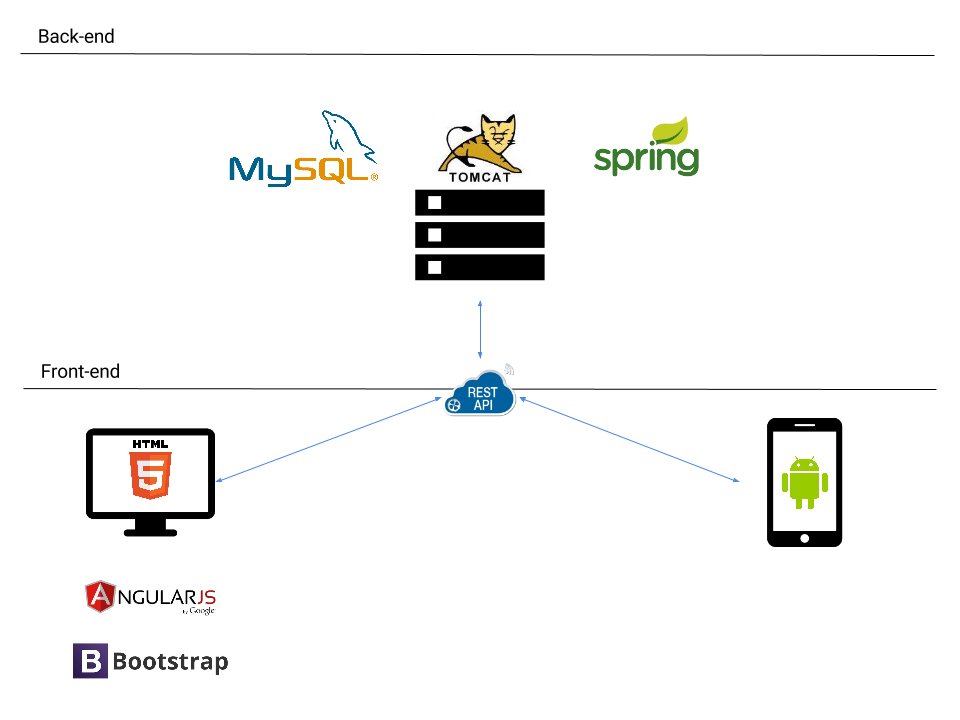
\includegraphics[width=\textwidth]{technologie_stack}
  \caption{Systeemarchitectuur}
  \label{fig:Systeemarchitectuur}
\end{figure}

De back-end wordt geïmplementeerd in Java, met behulp van het \textit{Spring Framework} \cite{Spring}. Voor de webapplicatie worden het \textit{AngularJS Framework} \cite{AngularJS} en het \textit{Bootstrap Framework} \cite{Bootstrap} gebruikt. De mobiele applicatie is beschikbaar voor het Android platform en wordt opnieuw in Java geïmplementeerd. De interactie tussen de front-end en back-end gebeurt door middel van zogenoemde \textit{RESTful} communicatie \cite{REST}. MySQL \cite{MySQL} dient als databasemanagementsysteem en wordt samen met de back-end gehost op een \textit{Tomcat} \cite{Tomcat} server.

\newpage
\subsection{Motivatie}
\begin{description}
    \item[Java] is een volwaardige objectgeoriënteerde programmeertaal waarmee alle leden van het ontwikkelingsteam ervaring hebben. Java beschikt over een groot aantal uitgebreide frameworks voor quasi alle denkbare toepassingen.
    \item[MySQL] is een vrij te gebruiken relationeel databasemanagementsysteem. Dit is ook het databasesysteem waarmee we het ontwikkelingsteam het best bekend is.
    \item[Spring Framework] is een een antwoord op de kritiek die gericht is aan de werking van het klassieke Java EE. Een van de grote sterktes is de uitgebreide documentatie.
    \item[Angular JS Framework] is een framework gebaseerd op JavaScript en dient als communicatiemiddel tussen back-end en front-end. Het is eenvoudig en handig voor snelle ontwikkeling van web pagina's. Ook is het makkelijk te combineren met HTML en CSS en is het compatibel met andere frameworks of libraries (bv. Bootstrap).
    \item[Bootstrap Framework] is een van de meest populaire HTML, CSS en JavaScript frameworks gebruikt voor de ontwikkeling van responsieve webapplicaties. Bootstrap maakt front-end web ontwikkeling sneller en makkelijker, het is flexibel en het levert zowel op desktop- als op mobiele platformen mooie resultaten op.
\end{description}

\clearpage
\section{Use cases} \label{sec:use_cases}
%%%%%%%%%%%%%%%
% MOBIELE APP %
%%%%%%%%%%%%%%%

% leerlingen VIEW
% agenda
%     lessen
%     notities
% berichten
% meldingen
%     alles
%     filters
% bestanden
% taken
% voortgang
%     BGV
%     PAV
% -----------
% profiel

% OUDERS VIEW
% kind kiezen
%     agenda
%     berichten
%     meldingen
%         alles
%         filters
%     taken (read only)
%     voortgang
%         BGV
%         PAV
% -----------
% profiel

% PERSONEEL MOBIELE VIEW
% agenda
%     lessen
%     notities
% berichten
% meldingen
%     alles
%     filters
% bestanden


%%%%%%%%%%%
% WEB APP %
%%%%%%%%%%%

% LEERKRACHT VIEW
% agenda
%     lessen
%     notities
% berichten
% meldingen
%     alles
%     filters
% bestanden
% puntenboek
%     vak kiezen
%     sorteren op klas, competentie, richting en zoeken op leerlingen
%     attitudes
%     rapporten printen
% klasbeheer
% vakken
%     Taakbeheer

% SYSTEEMBEHEERDER VIEW
% agenda
%     lessenrooster
%     notities
% berichten
% meldingen
%     alles
%     filters
% bestanden
% gebruikersbeheer (inschrijvingen, ...)
% werkgeversbeheer
% puntenboek
%     vak kiezen
%     sorteren op klas, competentie, richting en zoeken op leerlingen
%     rapporten printen
% opleidingbeheer (nieuwe opleidingen aanmaken, vakken hieraan koppelen vb het vak pav en een bepaald BGV traject, dit doen we voor de uitbreidbaarheid naar theorie vakken als technisch onderwijs dit systeem wilt gebruiken)

\subsection{Beheerder}
\begin{usecase}
    \addtitle{Use Case 1}{Agenda beheren} 
    \additemizedfield{Actoren}{
    	\item Beheerder
    }
    \addscenario{Beschrijving}{
        \item[] \textbf{Hoofdscenario:} \\
        Beheerder meldt zich aan via de webapplicatie en kiest om de agenda te bekijken. Systeem toont de agenda, waarin lessen en taken zijn opgenomen.\\
        \item[] \textbf{Alternatieve scenarios:} \\
        Beheerder kan zich ook via de mobiele applicatie aanmelden.\\
    }
\end{usecase}

% Berichten bekijken
\begin{usecase}
    \addtitle{Use Case 2}{Berichten bekijken} 
    \additemizedfield{Actoren}{
    	\item Beheerder
    }
    \addscenario{Beschrijving}{
        \item[] \textbf{Hoofdscenario:} \\
        Beheerder meldt zich aan via de webapplicatie. Beheerder kiest om de berichten te bekijken. Systeem toont berichten gericht aan de Beheerder. Het systeem biedt de mogelijkheid om te antwoorden op een bericht, een bericht te verwijderen, ...\\
       \item[] \textbf{Alternatieve scenarios:} \\
        Ouder kan zich ook via mobiele applicatie aanmelden.\\
    }
\end{usecase}

\clearpage
% Voortgang bekijken
\begin{usecase}
    \addtitle{Use Case 3}{Voortgang bekijken} 
    \additemizedfield{Actoren}{
    	\item Beheerder
    }
    \addscenario{Beschrijving}{
        \item[] \textbf{Hoofdscenario:} \\
        Beheerder meldt zich aan via de webapplicatie. Beheerder kiest om de voortgang te bekijken. Systeem geeft een overzicht (tussentijds rapport).\\
    }
\end{usecase}

% Bestanden beheren
\begin{usecase}
    \addtitle{Use Case 4}{Bestanden beheren} 
    \additemizedfield{Actoren}{
    	\item Beheerder
    }
    \addscenario{Beschrijving}{
        \item[] \textbf{Hoofdscenario:} \\
        Beheerder meldt zich aan via de webapplicatie. Beheerder kiest om zijn/haar documenten te bekijken. Systeem toont een overzicht van de aanwezige documenten. Beheerder kiest ervoor om bestanden te uploaden, verwijderen of bekijken.\\
        \item[] \textbf{Alternatieve scenarios:} \\
        Beheerder kan zich ook via mobiele applicatie aanmelden.\\
    }
\end{usecase}

% Gebruikers beheren
\begin{usecase}
    \addtitle{Use Case 5}{Gebruikers beheren} 
    \additemizedfield{Actoren}{
    	\item Beheerder
    }
    \addscenario{Beschrijving}{
        \item[] \textbf{Hoofdscenario:} \\
        Beheerder meldt zich aan via de webapplicatie. Beheerder kiest ervoor om gebruikers te beheren. Hier kan de beheerder gebruikers toevoegen, verwijderen, bewerken en op (in)actief zetten. De informatie die ingevuld kan worden is de naam, adres, geboortedatum, ... De inschrijvingsgerelateerde informatie is de graad waar de leerling in zit en de opleiding.\\
    }
\end{usecase}

% Opleidingen beheren
\begin{usecase}
    \addtitle{Use Case 6}{Opleidingen beheren} 
    \additemizedfield{Actoren}{
    	\item Beheerder
    }
    \addscenario{Beschrijving}{
        \item[] \textbf{Hoofdscenario:} \\
        Beheerder meldt zich aan via de webapplicatie. Beheerder kiest ervoor om opleidingen te beheren. Hier kan de beheerder opleidingen toevoegen, verwijderen of bewerken. De opleiding bestaat uit verschillende vakken (bv. PAV en BGV) en ieder vak bestaat uit verschillende competenties/doelstellingen. Competenties/doelstellingen kunnen toegevoegd, bewerkt en verwijderd worden.\\
    }
\end{usecase}

% Graden beheren
\begin{usecase}
    \addtitle{Use Case 7}{Graden beheren} 
    \additemizedfield{Actoren}{
    	\item Beheerder
    }
    \addscenario{Beschrijving}{
        \item[] \textbf{Hoofdscenario:} \\
        Beheerder meldt zich aan via de webapplicatie. Beheerder kiest ervoor om graden te beheren. Hier kan de beheerder graden toevoegen, verwijderen of bewerken.\\
    }
\end{usecase}

% Wergevers beheren
\begin{usecase}
    \addtitle{Use Case 8}{Werkgevers beheren} 
    \additemizedfield{Actoren}{
    	\item Beheerder
    }
    \addscenario{Beschrijving}{
        \item[] \textbf{Hoofdscenario:} \\
        Beheerder meldt zich aan via de webapplicatie. Beheerder kiest ervoor om werkgevers te beheren. Hier kan de beheerder werkgevers toevoegen, verwijderen of bewerken. De informatie die ingevuld kan worden is de naam van het bedrijf, telefoonnummer, adres, contactpersoon, ...\\
    }
\end{usecase}

\begin{figure}[H]
  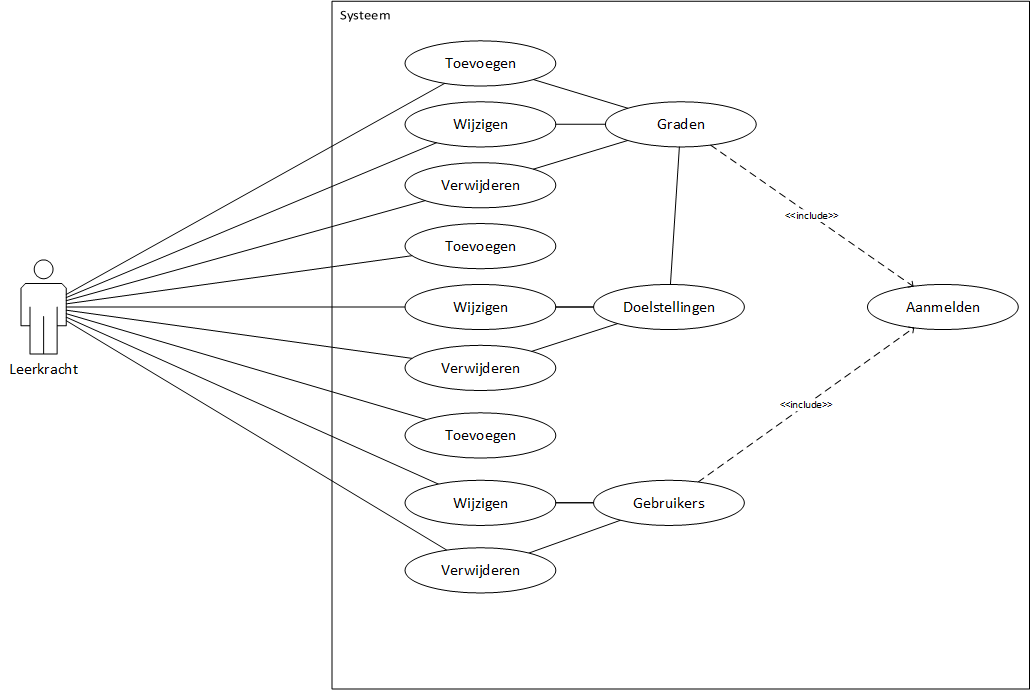
\includegraphics[width=\textwidth]{uc_beheerder}
  \caption{Usecase diagram voor de beheerder}
  \label{fig:usecase_beheerder}
\end{figure}


%%%%%%%%%%%%%%%%%%%%%%%%%%%%%%%%%%%%%%%%%%%%%%%%%%%%%%%%%%%%%%%%%%%%%%%%%%%%%
\clearpage
\subsection{Leerkracht}
\begin{usecase}
    \addtitle{Use Case 1}{Agenda bekijken} 
    \additemizedfield{Actoren}{
    	\item Leerkracht
    }
    \addscenario{Beschrijving}{
        \item[] \textbf{Hoofdscenario:} \\
        Leerkracht meldt zich aan via de webapplicatie en kiest om de agenda te bekijken. Systeem toont de agenda, waarin lessen zijn opgenomen.\\
        \item[] \textbf{Alternatieve scenarios:} \\
        Leerkracht kan zich ook via de mobiele applicatie aanmelden.\\
    }
\end{usecase}

% Berichten bekijken
\begin{usecase}
    \addtitle{Use Case 2}{Berichten bekijken} 
    \additemizedfield{Actoren}{
    	\item Leerkracht
    }
    \addscenario{Beschrijving}{
        \item[] \textbf{Hoofdscenario:} \\
        Leerkracht meldt zich aan via de webapplicatie. Leerkracht kiest om de berichten te bekijken. Systeem toont berichten gericht aan de leerkracht. Het systeem biedt de mogelijkheid om te antwoorden op een bericht, een bericht te verwijderen, ...\\
       \item[] \textbf{Alternatieve scenarios:} \\
        Leerkracht kan zich ook via mobiele applicatie aanmelden.\\
    }
\end{usecase}

\clearpage
% Taken beheren
\begin{usecase}
    \addtitle{Use Case 3}{Taak beheren} 
    \additemizedfield{Actoren}{
    	\item Leerkracht
    }
    \addscenario{Beschrijving}{
        \item[] \textbf{Hoofdscenario:} \\
        Leerkracht meldt zich aan via de webapplicatie. Leerkracht kiest het vak (bv. PAV of BGV). Systeem toont een overzicht van taken. Leekracht kiest ervoor om een nieuwe taak aan te maken. Leerkracht vult de informatie in en kiest welke leerlingen en/of klassen deze taak moeten maken.\\
       \item[] \textbf{Alternatieve scenarios:} \\
        Leerkracht kan taken verwijderen uit de lijst van taken.\\
    }
\end{usecase}

% Puntenboek
\begin{usecase}
    \addtitle{Use Case 4}{Puntenboek} 
    \additemizedfield{Actoren}{
    	\item Leerkracht
    }
    \addscenario{Beschrijving}{
        \item[] \textbf{Hoofdscenario:} \\
        Leerkracht meldt zich aan via de webapplicatie. Leerkracht  kiest ``Puntenboek''. Leerkracht kiest het vak dat door deze leerkracht gegeven wordt. Leerkracht kiest een leerling en geeft deze een score. Hier wordt ook feedback bij gegeven voor de leerling. De leerkracht kan kiezen om een rapport te genereren en af te drukken.\\ 
        \item[] \textbf{Alternatieve scenarios:} \\
        Indien de leerkracht er voor kiest om te quoteren op basis van een gekozen competentie/doelstelling, kan de leerkracht meerdere leerlingen tegelijk quoteren.\\
        Indien de competentie/doelstelling drie maal behaald werd, wordt deze automatisch geblokkeerd.\\
        Indien de leerkracht het jaaroverzicht van de leerling opvraagt, toont het systeem de score competentie per week.\\
        Indien de leerkracht er voor kiest om de attitudes van de leerling te quoteren, toont het systeem een overzicht per leerling.
    }
\end{usecase}

\clearpage
% Bestanden beheren
\begin{usecase}
    \addtitle{Use Case 5}{Bestanden beheren} 
    \additemizedfield{Actoren}{
    	\item Leerkracht
    }
    \addscenario{Beschrijving}{
        \item[] \textbf{Hoofdscenario:} \\
        Leerkracht meldt zich aan via de webapplicatie. Leerkracht kiest om zijn/haar documenten te bekijken. Systeem toont een overzicht van de aanwezige documenten. Leerkracht kiest ervoor om bestanden te uploaden, verwijderen of bekijken.\\
        \item[] \textbf{Alternatieve scenarios:} \\
        Leerkracht kan zich ook via mobiele applicatie aanmelden.\\
    }
\end{usecase}

% Klasbeer
\begin{usecase}
    \addtitle{Use Case 6}{Klasbeheer} 
    \additemizedfield{Actoren}{
    	\item Leerkracht
    }
    \addscenario{Beschrijving}{
        \item[] \textbf{Hoofdscenario:} \\
        Leerkracht meldt zich aan via de webapplicatie. Leerkracht kiest één van de opleidingen en het systeem toont een overzicht van de klassen. De leerkracht creëert een nieuwe klas, en voegt de gewenste leerlingen toe.\\
    }
\end{usecase}

\begin{figure}[H]
  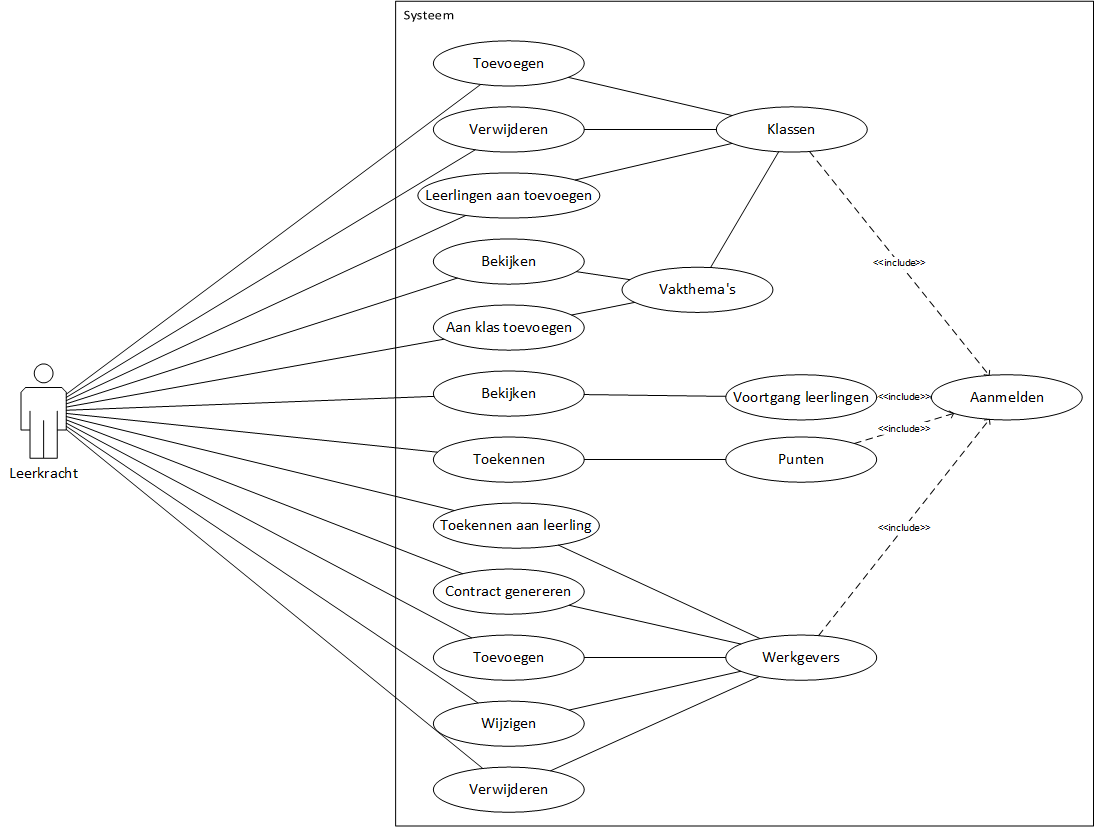
\includegraphics[width=\textwidth]{uc_leerkracht}
  \caption{Usecase diagram voor de leerkracht}
  \label{fig:usecase_leerkracht}
\end{figure}

%%%%%%%%%%%%%%%%%%%%%%%%%%%%%%%%%%%%%%%%%%%%%%%%%%%%%%%%%%%%%%%%%%%%%%%%%%%%%

\clearpage
\subsection{Leerling}
\begin{usecase}
    \addtitle{Use Case 1}{Agenda bekijken} 
    \additemizedfield{Actoren}{
    	\item Leerling
    }
    \addscenario{Beschrijving}{
        \item[] \textbf{Hoofdscenario:} \\
        Leerling meldt zich aan via de webapplicatie en kiest om de agenda te bekijken. Systeem toont de agenda, waarin lessen en taken zijn opgenomen.\\
        \item[] \textbf{Alternatieve scenarios:} \\
        Leerling kan zich ook via de mobiele applicatie aanmelden.\\
    }
\end{usecase}

% Berichten bekijken
\begin{usecase}
    \addtitle{Use Case 2}{Berichten bekijken} 
    \additemizedfield{Actoren}{
    	\item Leerling
    }
    \addscenario{Beschrijving}{
        \item[] \textbf{Hoofdscenario:} \\
        Leerling meldt zich aan via de webapplicatie. Leerling kiest om de berichten te bekijken. Systeem toont berichten gericht aan de leerling. Het systeem biedt de mogelijkheid om te antwoorden op een bericht, een bericht te verwijderen, ...\\
       \item[] \textbf{Alternatieve scenarios:} \\
    Ouder kan zich ook via mobiele applicatie aanmelden.\\
    Indien een ouder meerdere kinderen heeft op de school, moet eerst het gewenste kind gekozen worden.\\
    }
\end{usecase}

\clearpage
% Taken bekijken
\begin{usecase}
    \addtitle{Use Case 3}{Taken beheren} 
    \additemizedfield{Actoren}{
    	\item Leerling
    }
    \addscenario{Beschrijving}{
        \item[] \textbf{Hoofdscenario:} \\
        Leerling meldt zich aan via de webapplicatie. Leerling kiest om de taken te bekijken. Systeem toont een overzicht van toekomstige taken. Reeds ingestuurde taken kunnen bekeken worden. Leerling kiest up te loaden bestand uit ``mijn documenten''.\\
        \item[] \textbf{Alternatieve scenarios:} \\
        Leerling kan zich ook via mobiele applicatie aanmelden.\\
        Indien een ouder meerdere kinderen heeft op de school, moet eerst het gewenste kind gekozen worden.\\
        Leerling kan er voor kiezen om bestand vanop harde schijf te uploaden, i.p.v. uit ``mijn documenten''.
    }
\end{usecase}

% Voortgang bekijken
\begin{usecase}
    \addtitle{Use Case 4}{Voortgang bekijken} 
    \additemizedfield{Actoren}{
    	\item Ouder
    }
    \addscenario{Beschrijving}{
        \item[] \textbf{Hoofdscenario:} \\
        Leerling meldt zich aan via de webapplicatie. Leerling kiest om de voortgang te bekijken. Systeem geeft een overzicht (tussentijds rapport).\\
    \item[] \textbf{Alternatieve scenarios:} \\
        Leerling kan zich ook via mobiele applicatie aanmelden.\\
        Indien een ouder meerdere kinderen heeft op de school, moet eerst het gewenste kind gekozen worden.\\
    }
\end{usecase}

\clearpage
% Taken bekijken
\begin{usecase}
    \addtitle{Use Case 5}{Bestanden beheren} 
    \additemizedfield{Actoren}{
    	\item Leerling
    }
    \addscenario{Beschrijving}{
        \item[] \textbf{Hoofdscenario:} \\
        Leerling meldt zich aan via de webapplicatie. Leerling kiest om zijn/haar documenten te bekijken. Systeem toont een overzicht van de aanwezige documenten. Leerling kiest ervoor om bestanden te uploaden, verwijderen of bekijken.
        \item[] \textbf{Alternatieve scenarios:} \\
        Leerling kan zich ook via mobiele applicatie aanmelden.\\
    }
\end{usecase}

\begin{figure}[H]
  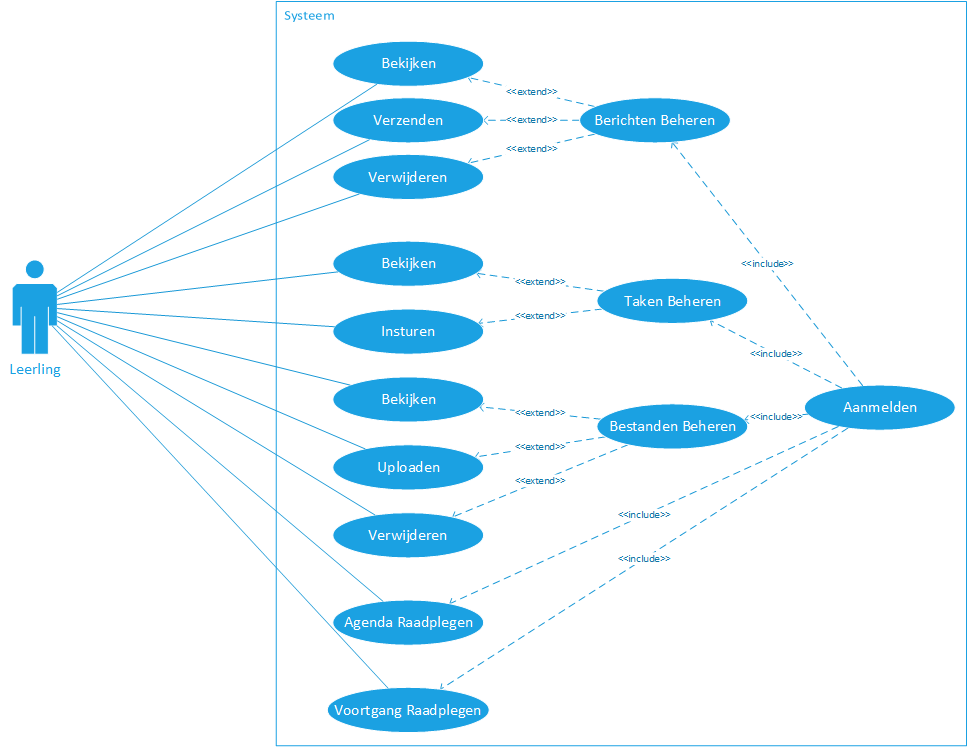
\includegraphics[width=\textwidth]{uc_leerling}
  \caption{Usecase diagram voor de leerling}
  \label{fig:usecase_leerling}
\end{figure}

%%%%%%%%%%%%%%%%%%%%%%%%%%%%%%%%%%%%%%%%%%%%%%%%%%%%%%%%%%%%%%%%%%%%%%%%%%%%%

\clearpage
\subsection{Ouder}
% Agenda van kind bekijken
\begin{usecase}
\addtitle{Use Case 1}{Agenda van kind bekijken} 
\additemizedfield{Actoren}{
	\item Ouder
}
\addscenario{Beschrijving}{
    \item[] \textbf{Hoofdscenario:} \\
    Ouder meldt zich aan via de webapplicatie. Ouder kiest om de agenda van het kind te bekijken. Systeem toont agenda, waarin lessen en taken zijn opgenomen.\\
    \item[] \textbf{Alternatieve scenarios:} \\
    Ouder kan zich ook via mobiele applicatie aanmelden.\\
    Indien een ouder meerdere kinderen heeft op de school, moet eerst het gewenste kind gekozen worden.\\
}
\end{usecase}

% Berichten bekijken
\begin{usecase}
\addtitle{Use Case 2}{Berichten bekijken} 
\additemizedfield{Actoren}{
	\item Ouder
}
\addscenario{Beschrijving}{
    \item[] \textbf{Hoofdscenario:} \\
    Ouder meldt zich aan via de webapplicatie. Ouder kiest om de berichten te bekijken. Systeem toont berichten gericht aan de ouder van het kind. Het systeem biedt de mogelijkheid om te antwoorden op een bericht, een bericht te verwijderen, ...\\
    \item[] \textbf{Alternatieve scenarios:} \\
    Ouder kan zich ook via mobiele applicatie aanmelden.\\
    Indien een ouder meerdere kinderen heeft op de school, moet eerst het gewenste kind gekozen worden.\\
}
\end{usecase}

\clearpage
% Taken bekijken
\begin{usecase}
\addtitle{Use Case 3}{Taken bekijken} 
\additemizedfield{Actoren}{
	\item Ouder
}
\addscenario{Beschrijving}{
    \item[] \textbf{Hoofdscenario:} \\
    Ouder meldt zich aan via de webapplicatie. Ouder kiest om de taken te bekijken. Systeem toont een overzicht van toekomstige taken. Reeds ingestuurde taken kunnen bekeken worden.\\
    \item[] \textbf{Alternatieve scenarios:} \\
    Ouder kan zich ook via mobiele applicatie aanmelden.\\
    Indien een ouder meerdere kinderen heeft op de school, moet eerst het gewenste kind gekozen worden.\\
}
\end{usecase}

% Voortgang bekijken
\begin{usecase}
\addtitle{Use Case 4}{Voortgang bekijken} 
\additemizedfield{Actoren}{
	\item Ouder
}
\addscenario{Beschrijving}{
    \item[] \textbf{Hoofdscenario:} \\
    Ouder meldt zich aan via de webapplicatie. Ouder kiest om de voortgang van het kind te bekijken. Systeem geeft een overzicht (tussentijds rapport).\\
    \item[] \textbf{Alternatieve scenarios:} \\
    Ouder kan zich ook via mobiele applicatie aanmelden.\\
    Indien een ouder meerdere kinderen heeft op de school, moet eerst het gewenste kind gekozen worden.\\
}
\end{usecase}

\begin{figure}[H]
  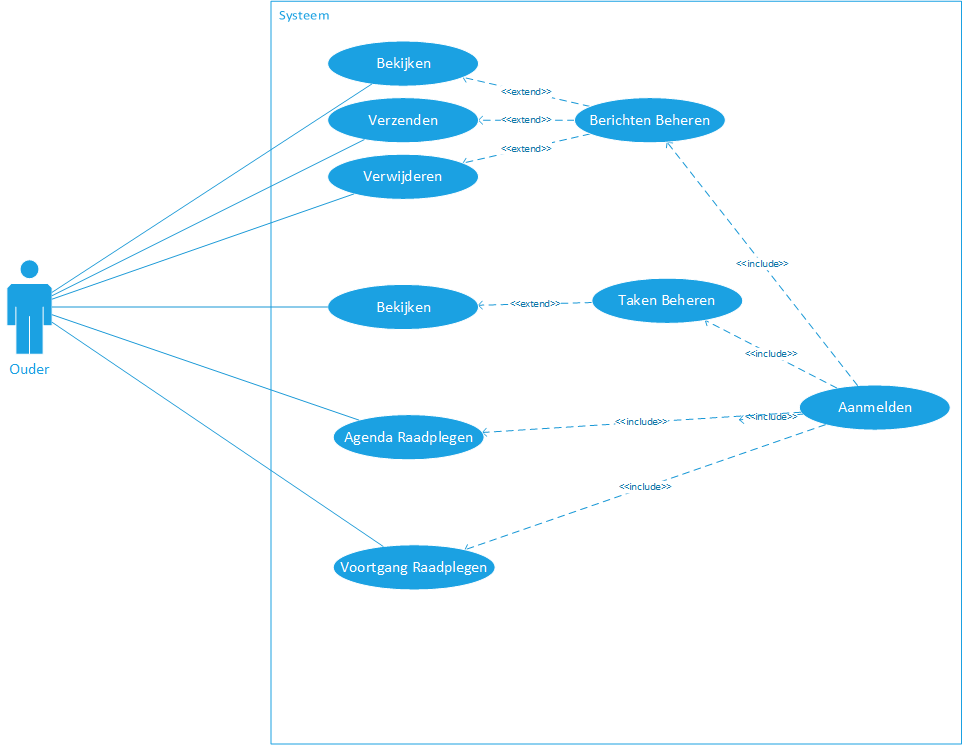
\includegraphics[width=\textwidth]{uc_ouder}
  \caption{Usecase diagram voor de ouder}
  \label{fig:usecase_ouder}
\end{figure}


\newpage
\begin{appendices}
\section{Mockups webapplicatie}

\begin{figure}[H]
  \centerline{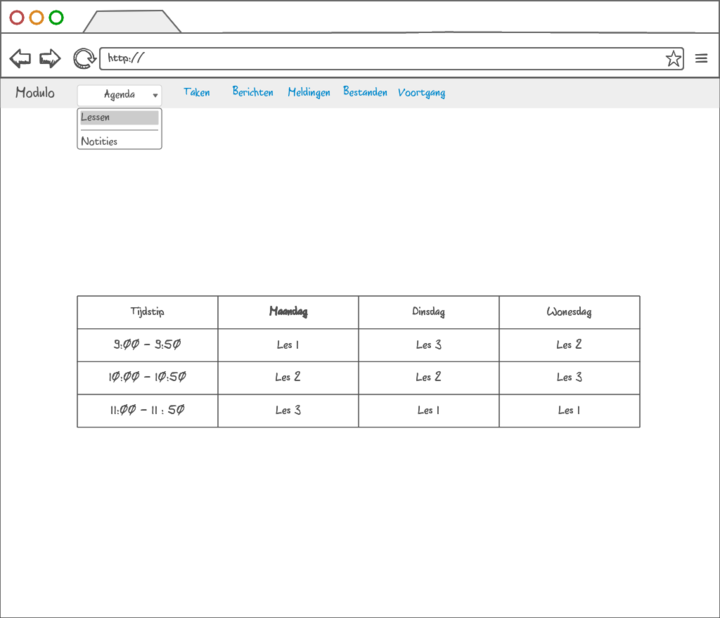
\includegraphics[width=\textwidth]{web}}
  \caption{Webapplicatie}
  \label{fig:web}
\end{figure}

\newpage
\section{Mockups mobiele applicatie}

\begin{figure}[H]
  \centerline{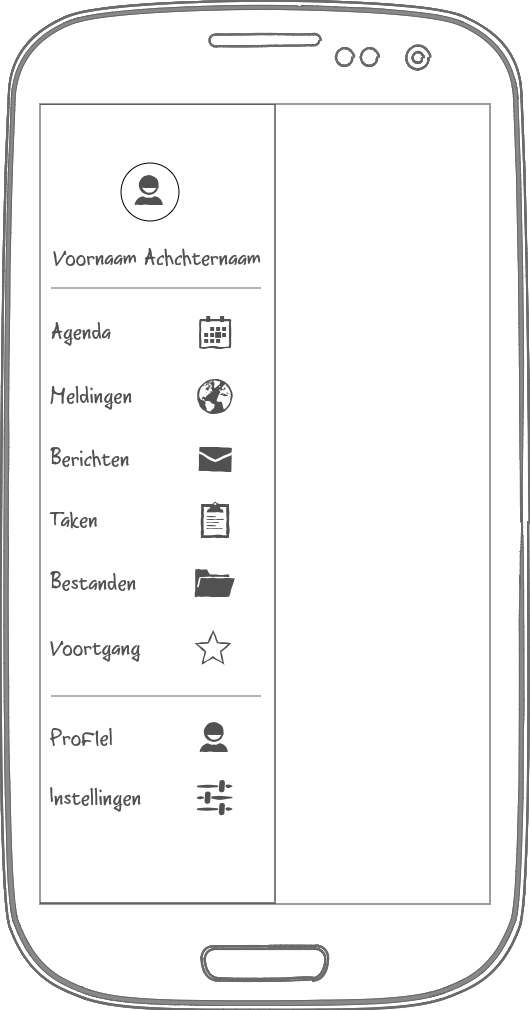
\includegraphics[width=\textwidth*4/5]{mobiel_leerling}}
  \caption{Menu voor leerlingen}
  \label{fig:mobiel_leerling}
\end{figure}

\newpage
\begin{figure}[H]
  \centerline{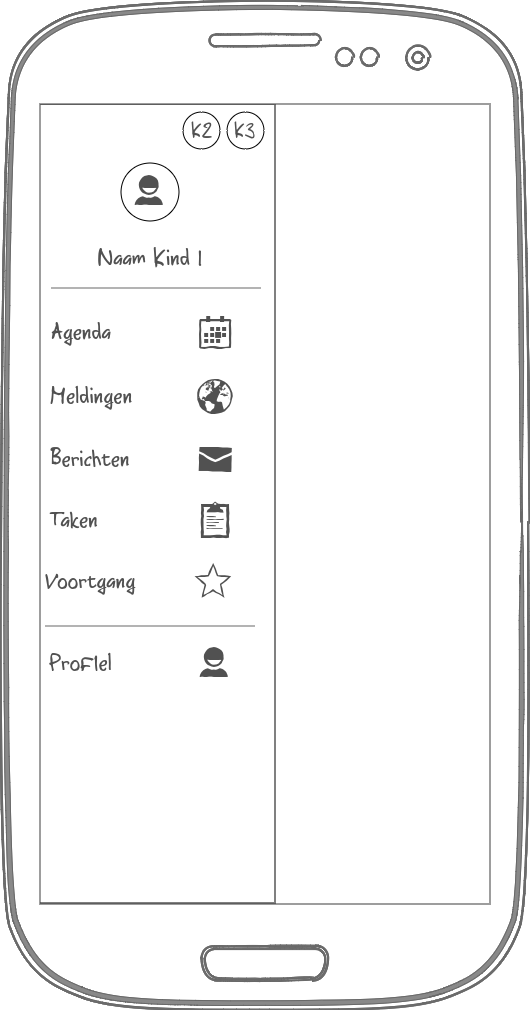
\includegraphics[width=\textwidth*4/5]{mobiel_ouder}}
  \caption{Menu voor ouders}
  \label{fig:mobiel_ouder}
\end{figure}

\newpage
\begin{figure}[H]
  \centerline{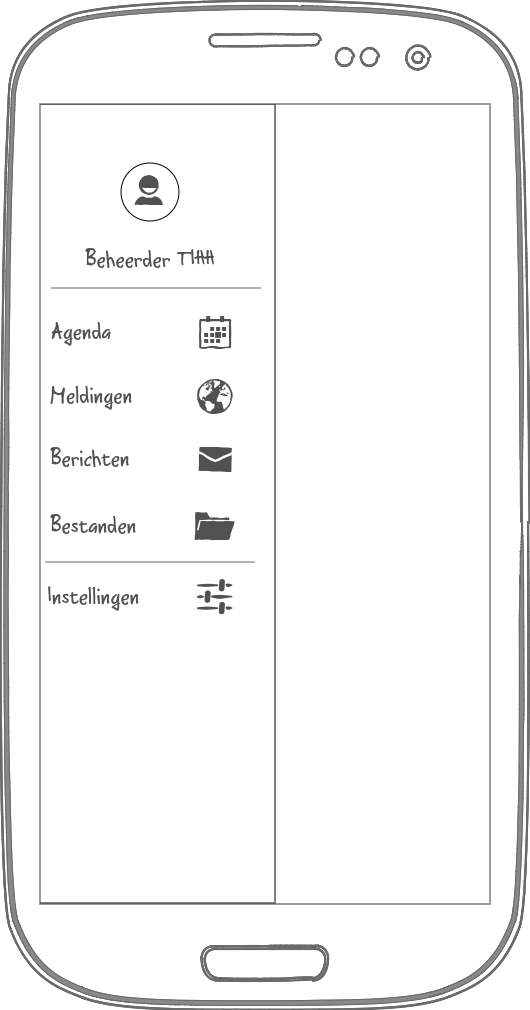
\includegraphics[width=\textwidth*4/5]{mobiel_personeel}}
  \caption{Menu voor personeel}
  \label{fig:mobiel_personeel}
\end{figure}

\begin{figure}[H]
  \centerline{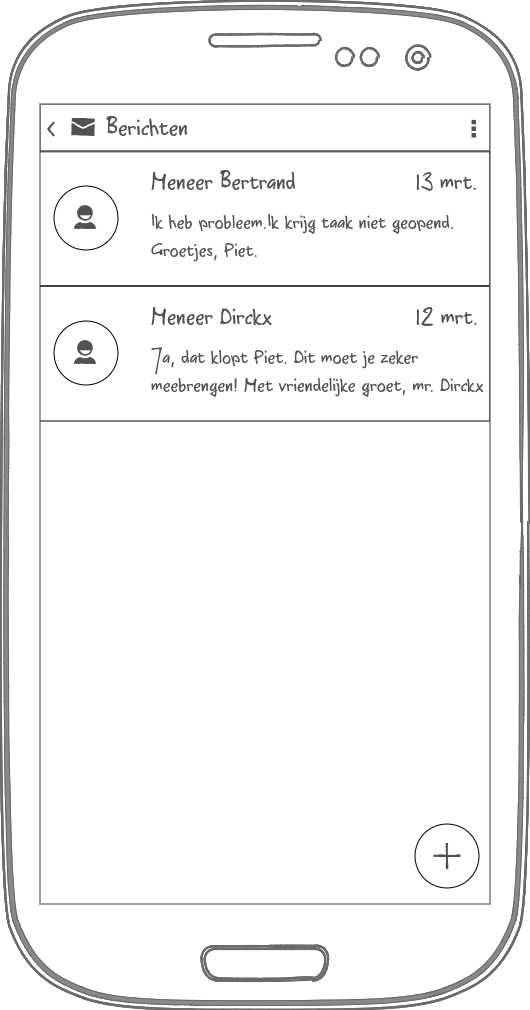
\includegraphics[width=\textwidth*4/5]{mobiel_berichten}}
  \caption{Berichten menu}
  \label{fig:mobiel_berichten}
\end{figure}

\newpage
\begin{figure}[H]
  \centerline{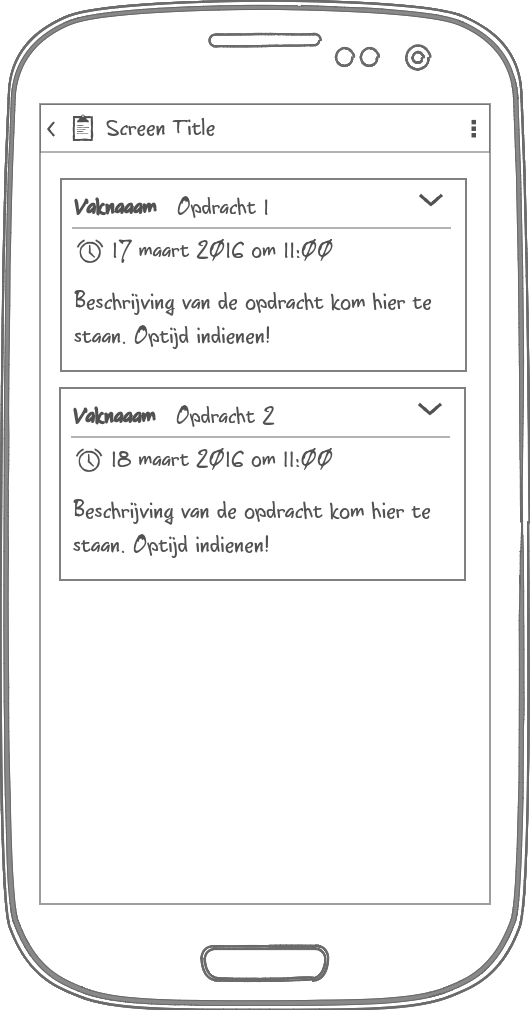
\includegraphics[width=\textwidth*4/5]{mobiel_taken}}
  \caption{Taken menu}
  \label{fig:mobiel_taken}
\end{figure}

\newpage
\begin{figure}[H]
  \centerline{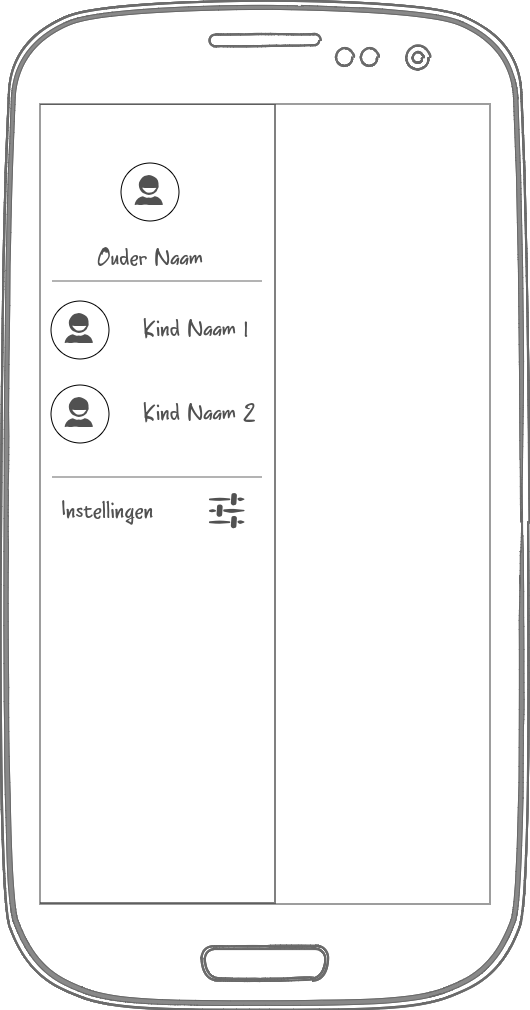
\includegraphics[width=\textwidth*4/5]{mobiel_kies_kind}}
  \caption{Ouder selecteert uit ingeschreven kinderen}
  \label{fig:mobiel_kies_kind}
\end{figure}

\end{appendices}

\newpage
\bibliography{Referenties}
\bibliographystyle{unsrt}

\end{document}
